\documentclass[11pt]{article}

% ---- Packages ----
\usepackage[a4paper,margin=1in]{geometry}
\usepackage{lmodern}
\usepackage[T1]{fontenc}
\usepackage{microtype}
\usepackage{amsmath,amssymb,amsthm}
\usepackage{graphicx}
\usepackage{booktabs}
\usepackage{xcolor}
\usepackage{enumitem}
\usepackage{verbatim}
\usepackage{listings}
\usepackage[colorlinks=true,allcolors=teal!60!black]{hyperref}
\usepackage{natbib}
\bibliographystyle{plainnat}

% ---- Minimal algorithm formatting ----
\newenvironment{algorithm}[1][t]{\begin{figure}[#1]\rule{\linewidth}{0.5pt}\par}{%
  \par\rule{\linewidth}{0.5pt}\end{figure}}

\newtheorem{definition}{Definition}
\newtheorem{proposition}{Proposition}
\newtheorem{theorem}{Theorem}

\lstset{basicstyle=\ttfamily\small,breaklines=true,columns=fullflexible,
        frame=single,framerule=0.3pt,xleftmargin=4pt,xrightmargin=4pt}

% =====================================================================
% RESULT MACROS: single source of truth, filled from results/*.json
% =====================================================================
% Defaults below are the real values from results/*.json (so the paper is
% correct even without _numbers.tex); scripts/paper_numbers.py regenerates
% _numbers.tex, which \renewcommand-overrides them identically.
% E1 content guard
\newcommand{\piTrace}{0.827}\newcommand{\piTraceSd}{0.036}
\newcommand{\piBest}{0.800}\newcommand{\piBestName}{LinearSVC}\newcommand{\piP}{0.028}
\newcommand{\piLat}{176}\newcommand{\piSize}{12.5}
\newcommand{\jbTrace}{0.967}\newcommand{\jbTraceSd}{0.005}
\newcommand{\jbBest}{0.982}\newcommand{\jbBestName}{LogReg}
\newcommand{\jbLat}{287}
% E2 behaviour: ASR (A) and FPR (F), per-call (Pc) vs TRACE (Tr), 4 families
\newcommand{\btExfPcA}{1.000}\newcommand{\btExfPcF}{0.000}\newcommand{\btExfTrA}{0.000}\newcommand{\btExfTrF}{0.000}
\newcommand{\btScoPcA}{0.000}\newcommand{\btScoPcF}{0.000}\newcommand{\btScoTrA}{0.000}\newcommand{\btScoTrF}{0.000}
\newcommand{\btAudPcA}{0.000}\newcommand{\btAudPcF}{1.000}\newcommand{\btAudTrA}{0.000}\newcommand{\btAudTrF}{0.048}
\newcommand{\btPriPcA}{0.000}\newcommand{\btPriPcF}{1.000}\newcommand{\btPriTrA}{0.000}\newcommand{\btPriTrF}{0.000}
% E3 ablation overall attack recall
\newcommand{\ablContent}{0.505}\newcommand{\ablBehavior}{0.667}\newcommand{\ablTrace}{0.911}
% E4 tamper / E5 systems
\newcommand{\tamperRate}{1.00}\newcommand{\verifyUs}{933}
\newcommand{\behLat}{4.90}\newcommand{\behMem}{322}
\newcommand{\ledgerBytes}{373}
% E5 content-guard latency at the deployed C=200 budget (median / p99, us)
\newcommand{\latMed}{107}\newcommand{\latPNN}{428}\newcommand{\latStd}{109}
% E6 robustness
\newcommand{\obfPlain}{0.733}\newcommand{\obfSpace}{0.721}
\newcommand{\transAin}{0.849}\newcommand{\transAcross}{0.713}
\newcommand{\transBin}{0.967}\newcommand{\transBcross}{0.209}
% Regenerate/override all of the above from results/*.json:
\IfFileExists{_numbers.tex}{% AUTO-GENERATED by scripts/paper_numbers.py. Do not edit by hand.
\renewcommand{\piTrace}{0.827}
\renewcommand{\piTraceSd}{0.036}
\renewcommand{\piLat}{176}
\renewcommand{\piSize}{12.5}
\renewcommand{\piBest}{0.800}
\renewcommand{\piBestName}{LinearSVC}
\renewcommand{\piP}{0.028}
\renewcommand{\jbTrace}{0.967}
\renewcommand{\jbTraceSd}{0.005}
\renewcommand{\jbLat}{287}
\renewcommand{\jbBest}{0.982}
\renewcommand{\jbBestName}{LogReg}
\renewcommand{\btExfPcA}{1.000}
\renewcommand{\btExfPcF}{0.000}
\renewcommand{\btExfTrA}{0.000}
\renewcommand{\btExfTrF}{0.000}
\renewcommand{\btAudPcA}{0.000}
\renewcommand{\btAudPcF}{1.000}
\renewcommand{\btAudTrA}{0.000}
\renewcommand{\btAudTrF}{0.048}
\renewcommand{\btPriPcA}{0.000}
\renewcommand{\btPriPcF}{1.000}
\renewcommand{\btPriTrA}{0.000}
\renewcommand{\btPriTrF}{0.000}
\renewcommand{\btScoPcA}{0.000}
\renewcommand{\btScoPcF}{0.000}
\renewcommand{\btScoTrA}{0.000}
\renewcommand{\btScoTrF}{0.000}
\renewcommand{\ablContent}{0.505}
\renewcommand{\ablBehavior}{0.667}
\renewcommand{\ablTrace}{0.911}
\renewcommand{\tamperRate}{1.00}
\renewcommand{\verifyUs}{933}
\renewcommand{\behLat}{4.90}
\renewcommand{\behMem}{322}
\renewcommand{\ledgerBytes}{373}
\renewcommand{\latMed}{107}
\renewcommand{\latPNN}{428}
\renewcommand{\latStd}{109}
\renewcommand{\obfPlain}{0.733}
\renewcommand{\obfSpace}{0.721}
\renewcommand{\transAin}{0.849}
\renewcommand{\transAcross}{0.713}
\renewcommand{\transBin}{0.967}
\renewcommand{\transBcross}{0.209}
}{}

% ---- Title ----
\title{\textbf{TRACE: A Tsetlin Runtime Assurance and Certification Engine\\
for Interpretable, Tamper-Evident Guardrails on Agentic AI}}
\author{Anwar Debes\\
University of Agder\\
\vspace{0.4em}\small Draft v1.0, June 2026}
\date{}

\begin{document}
\maketitle

\begin{abstract}
Large language model (LLM) agents now take consequential actions (reading
records, sending messages, moving money), yet the guardrails deployed to keep
them safe are, almost without exception, multi-billion-parameter neural
classifiers: accurate but opaque, GPU-bound, latency-unspecified, retrained at
data-centre cost, and, critically, producing no auditable record an external
party can verify. None of the eight production guardrails I survey exposes a
tamper-evident audit trail, and only one performs any formal reasoning (and that
over single facts, not behaviour over time). I present \textbf{TRACE}, a
Tsetlin Runtime Assurance and Certification Engine: a CPU-only, interpretable,
sub-millisecond (at its deployed clause budget) guardrail that wraps any agent
and emits, for every session, a
\emph{tamper-evident, independently-verifiable certificate} of what it checked.
TRACE has three components on one logic substrate, the Echo-Trace Tsetlin
Automaton of THGTM~\citep{debes2026thgtm}: (i) a \emph{content guard}, a Tsetlin
Machine whose learned clauses are human-readable conjunctions of tokens; (ii) a
\emph{behaviour guard}, a bank of online finite-trace-LTL monitors whose memory
is constant in the trajectory length and whose per-step cost is $O(1)$; and
(iii) a \emph{certificate ledger}, a hash-chained, HMAC-signed, Merkle-rooted
log that an auditor re-verifies without the model. On two real Apache-2.0
prompt-injection datasets the content guard reaches $\piTrace\pm\piTraceSd$ F1,
\emph{significantly above} the strongest CPU baseline ($\piBestName$ $\piBest$,
Mann-Whitney $p=\piP$), at a $\latMed\,\mu$s median ($\piLat\,\mu$s mean) per
check and $\piSize$\,KiB. On a
four-family trajectory benchmark the memoryless per-call paradigm is caught in a
bind: it either misses the attack entirely (slow-roll exfiltration: attack
success rate $1.0$) or can only catch it by flagging every benign session
(missing-audit and privilege: false-positive rate $1.0$), while TRACE's online
monitors achieve attack success rate $0$ at false-positive rate $\le 0.05$ on all
four. Six tamper classes against the ledger are detected at rate $\tamperRate$
and localised. I give a precise account of the guarantees (tamper-evidence and
symmetric authentication, not non-repudiation), an honest catalogue of failure
modes (distribution shift), and I position TRACE against both neural guardrails
and the 2025 agent-enforcement line. All numbers, figures
and certificates regenerate from the repository on a single CPU.
\end{abstract}

\section{Introduction}

The deployment surface of LLM agents has moved, in under two years, from
chatbots that emit text to autonomous systems that call tools, browse, write
code, and act on a user's behalf. With agency comes a safety problem that
single-turn content moderation does not capture: an agent is unsafe \emph{even
without an adversary} (the best undefended GPT-4o agent in
AgentDojo~\citep{debenedetti2024agentdojo} succumbs to a targeted
prompt-injection $47.7\%$ of the time on the ``important message'' attack), and
the most damaging attacks unfold \emph{over a trajectory}, not in a single call:
indirect prompt injection~\citep{greshake2023indirect}, slow-roll data
exfiltration, out-of-role tool use, and privilege escalation are all
behaviours the OWASP Top~10 for Agentic Applications~\citep{owasp2025agentic}
codifies.

At the same time, the regulatory floor is rising. The EU AI
Act~\citep{euaiact2024}, whose high-risk obligations apply from 2~August~2026,
requires high-risk systems to \emph{automatically log events over their
lifetime} (Article~12), to remain robust to data and model poisoning and
adversarial evasion (Article~15), to be overseeable by a human who can detect
anomalies and intervene (Article~14), and obliges deployers to retain those logs
for at least six months (Article~26). A guardrail that cannot produce an
auditable, tamper-evident record is, increasingly, not deployable.

\paragraph{The gap.} I surveyed eight production and research guardrails:
Llama~Guard~3/4~\citep{metallamaguard3,metallamaguard4},
ShieldGemma~\citep{zeng2024shieldgemma}, Granite
Guardian~\citep{ibm2024graniteguardian}, WildGuard~\citep{han2024wildguard},
Constitutional Classifiers~\citep{sharma2025constitutional}, NeMo
Guardrails~\citep{rebedea2023nemo}, and the managed Azure / AWS
services~\citep{azurepromptshields,awsbedrockguardrails}. They are strong
detectors, but they share four structural limitations. They are
\emph{black-box} (a $2$--$12$\,B-parameter forward pass, no human-readable
rationale); \emph{GPU-bound and latency-unspecified} (not one publishes a
per-decision latency); \emph{non-auditable} (none emits a cryptographic record
of its decisions); and \emph{per-call} (they classify one input or output, with
no notion of a temporal policy over a trajectory). None of the eight is
interpretable, CPU-cheap, cryptographically auditable, \emph{and} temporal.

\paragraph{Contribution.} TRACE fills exactly that gap with a guardrail built on
propositional logic rather than dense tensors. Its substrate is the
Echo-Trace Tsetlin Automaton (ETTA) from the prior THGTM
line~\citep{debes2026thgtm}, which makes every decision a Boolean clause over
named features and therefore auditable by construction. On that substrate I
build:

\begin{enumerate}[leftmargin=1.4em]
\item a \textbf{content guard} (\S\ref{sec:content}), a Tsetlin Machine that
classifies text (prompts, retrieved documents, tool arguments, outputs) as
benign or unsafe, whose clauses read like \texttt{IF ignore AND previous
$\rightarrow$ UNSAFE} and whose firing pattern is packaged as a CNF receipt;
\item a \textbf{behaviour guard} (\S\ref{sec:behavior}), a bank of online
monitors for a curated bounded fragment of finite-trace
LTL~\citep{bauer2011ltl3,degiacomo2013ltlf} (\textsc{Always}, \textsc{Never},
\textsc{BoundedCount}, \textsc{Response}, \textsc{Precedence}), each $O(1)$ or
$O(\text{window})$ per step and \emph{constant memory in the trajectory length};
\item a \textbf{certificate ledger} (\S\ref{sec:ledger}), a hash-chained,
HMAC-signed, Merkle-rooted audit log~\citep{schneier1998securelogs,
crosby2009historytree,laurie2013ct,krawczyk1997hmac} that an external auditor
re-verifies \emph{without the model};
\item \textbf{model-agnostic adapters} (\S\ref{sec:adapters}) that normalise
OpenAI, DeepSeek and Anthropic tool calls into the events the policy speaks in,
so one policy moves unchanged across agents.
\end{enumerate}

\paragraph{What I claim and what I do not.} I do \emph{not} claim to beat
multi-billion-parameter GPU guardrails on raw multilingual detection accuracy;
their published numbers (Table~\ref{tab:guardrails}) are reported for context
and were measured on different data. I claim that TRACE is the first guardrail
to combine interpretability, CPU-only sub-millisecond operation, cryptographic
auditability, and temporal-trajectory verification in one system, and I back
each adjective with a measurement or a proof. I am explicit about the
guarantees I provide (tamper-\emph{evidence} and symmetric authentication, not
non-repudiation; \S\ref{sec:ledger}) and about where TRACE breaks
(distribution shift; \S\ref{sec:robust}).

\paragraph{Reproducibility.} Every number, figure and certificate in this paper
is produced by code in the accompanying repository on a single CPU; the two
datasets are Apache-2.0 and vendored at a pinned revision. The full experiment
suite runs in minutes with \texttt{make reproduce}.

\section{Background and related work}
\label{sec:related}

\paragraph{Tsetlin Machines.} A Tsetlin Automaton~\citep{granmo2018tsetlin} is a
two-action finite-state learner; a Tsetlin Machine (TM) is a team of automata
that learns a set of \emph{clauses}, each a conjunction of literals (a feature
or its negation), whose votes are thresholded into a class. TMs are natively
interpretable, train online, and run in fixed-point logic, which has yielded
ASIC accelerators at $8.6$\,nJ/frame for MNIST~\citep{tunheim2025asic} and
$16.58\,\mu$W for keyword spotting~\citep{lin2025tsetlinkws,lei2021kws}; integer
weights~\citep{abeyrathna2020integer}, clause sharing~\citep{glimsdal2021coalesced},
convolution~\citep{granmo2019convolutional}, graphs~\citep{granmo2025graph} and
explainable NLP~\citep{bhattarai2020novelty,bhattarai2021fakenews} extend the
family. THGTM~\citep{debes2026thgtm} adds the Echo-Trace automaton (a TA with
one eligibility-trace float) for temporal credit assignment and introduces
per-clause CNF receipts. \emph{No prior TM work addresses LLM guardrails, agent
safety, or hallucination detection}; TRACE is, to my knowledge, the first.

\paragraph{LLM and agent guardrails.} The dominant paradigm is a fine-tuned LLM
classifier (Table~\ref{tab:guardrails}). These are effective but opaque,
GPU-resident, and, by my survey, uniformly latency-unspecified and
non-auditable. NeMo Guardrails~\citep{rebedea2023nemo} adds a programmable-rails
DSL but delegates classification to LLMs. Managed services
\citep{azurepromptshields,awsbedrockguardrails} hide the model entirely; the lone
exception that performs any formal reasoning is AWS's Automated Reasoning checks,
which verify the factual policy-consistency of an individual output rather than
behaviour over a trajectory. TRACE differs on every axis except that it, too, is
a learned detector.

\paragraph{Agent attacks and benchmarks.} AgentDojo~\citep{debenedetti2024agentdojo},
InjecAgent~\citep{zhan2024injecagent}, and AgentHarm~\citep{andriushchenko2024agentharm}
benchmark prompt-injection and harmful-tool-use against agents;
Greshake~et~al.~\citep{greshake2023indirect} introduced indirect injection; OWASP
\citep{owasp2025agentic} codifies the agentic threat classes. I use these
taxonomies to ground (and to scope) my trajectory benchmark.

\paragraph{Runtime verification.} Monitoring a system against a temporal
specification is the subject of runtime verification (RV). Bauer, Leucker and
Schallhart~\citep{bauer2011ltl3} give the canonical three-valued LTL monitor: a
deterministic automaton, $O(1)$ per event after an offline construction that is
double-exponential in the formula. De~Giacomo and Vardi~\citep{degiacomo2013ltlf}
formalise LTL over finite traces (LTLf). TRACE deliberately restricts itself to a
\emph{fixed library} of bounded patterns rather than compiling arbitrary LTL,
trading expressiveness for a guaranteed constant-per-step cost with \emph{no}
automaton-construction blow-up (\S\ref{sec:behavior}).

\paragraph{Agent runtime enforcement.} Closest to TRACE is the 2025
agent-enforcement line: AgentSpec~\citep{wang2025agentspec} (a rule DSL),
ProGuard~\citep{wang2025proguard} (probabilistic model checking), and
Agent-C~\citep{kamath2025agentc} (SMT over temporal constraints). These enforce
behaviour but differ in mechanism and, crucially, none couples enforcement with
an \emph{interpretable learned content detector} and a \emph{cryptographic
certificate} of the session. TRACE's monitors are simpler by design (deterministic,
constant-per-step) and its contribution is the end-to-end \emph{certifying}
engine, not a new logic.

\paragraph{Tamper-evident logging.} The certificate ledger is a direct
application of secure-log constructions: hash chaining and forward-secure MACs
\citep{schneier1998securelogs}, history trees~\citep{crosby2009historytree},
Certificate Transparency's Merkle logs~\citep{laurie2013ct}, and
HMAC~\citep{krawczyk1997hmac}. My contribution is not the cryptography but its
application to per-decision agent governance.

\begin{table}[t]\centering\small
\caption{Production / research guardrails vs.\ TRACE. ``Lat.'' = a published
per-decision latency. None of the surveyed systems is interpretable, CPU-only,
auditable, \emph{and} temporal. Guardrail figures are from the cited model cards
/ papers and were measured on heterogeneous data; they are context, not a
head-to-head comparison.}
\label{tab:guardrails}
\begin{tabular}{lccccc}
\toprule
System & Params & Interp. & CPU/Lat. & Crypto audit & Temporal \\
\midrule
Llama Guard 3/4 & 8/12\,B & no & GPU / -- & no & no \\
ShieldGemma & 2--27\,B & no & GPU / -- & no & no \\
Granite Guardian & 2/8\,B & no & GPU / -- & no & no \\
WildGuard & 7\,B & no & GPU / -- & no & no \\
Constitutional Classifiers & LLM-scale & no & GPU / -- & no & no \\
NeMo Guardrails & LLM-scale & rails & GPU / -- & no & partial \\
Azure / AWS (managed) & undisclosed & no & cloud / -- & no & no \\
\midrule
AgentSpec / ProGuard / Agent-C & n/a & rules & CPU / ms & no & \textbf{yes} \\
\textbf{TRACE (this work)} & \textbf{12.5\,KiB} & \textbf{yes} & \textbf{CPU / $\mu$s} & \textbf{yes} & \textbf{yes} \\
\bottomrule
\end{tabular}
\end{table}

\section{Threat model}
\label{sec:threat}

\paragraph{Setting.} An agent executes a sequence of steps; at each step it
consumes text (user input, retrieved content, tool output) and may issue a tool
call. TRACE sits inline: it sees each text and each tool call, in either
\emph{monitor} mode (record only) or \emph{enforce} mode (it may block).

\paragraph{Adversary.} I consider an adversary who (a) injects malicious
instructions directly into a prompt or indirectly via retrieved
content~\citep{greshake2023indirect}, aiming to redirect the agent; and (b)
drives the agent toward harmful \emph{trajectories}: exfiltrating data over
many small steps, acting out of role, omitting required audit logging, or
performing privileged actions without authorisation. These map to the OWASP
agentic classes of goal hijacking, tool misuse, and identity/privilege
abuse~\citep{owasp2025agentic}. I additionally consider an adversary who, after
the fact, tampers with the audit log to hide what happened.

\paragraph{What TRACE defends.} (i) Injection attempts whose surface form
resembles training examples are caught by the content guard. (ii) Any trajectory
violating a declared temporal policy is caught by the behaviour guard,
\emph{including} attacks that are invisible to per-call inspection. (iii) Any
post-hoc modification, insertion, deletion, or reordering of log entries is
detected by ledger verification.

\paragraph{What TRACE does not defend.} The content guard is a learned detector
and inherits the usual failure modes: \emph{novel or out-of-distribution}
injections that do not resemble the training data evade it (\S\ref{sec:robust});
I quantify this rather than hide it. The behaviour guard only enforces \emph{declared} policies;
a harmful behaviour nobody wrote a policy for is not caught. TRACE assumes the
verification key is secret and the inline engine itself is not compromised
(if the engine is compromised, no inline guardrail helps). Tamper-evidence is
\emph{detection}, not prevention: an attacker who controls storage can delete the
whole log, but cannot alter a signed certificate undetectably.

\section{The TRACE architecture}
\label{sec:arch}

All three components share one substrate. An Echo-Trace Tsetlin Automaton is a
standard two-action TA with $N$ states per action augmented with one
eligibility-trace float; with the trace disabled it is a vanilla
TA~\citep{granmo2018tsetlin}. The content guard runs in this vanilla regime
(i.i.d.\ text); the trace is available for bounded-history features. Using a
single logic substrate means every decision TRACE certifies (content or
behaviour) has the same inspectable, replayable semantics.

\subsection{Content guard}
\label{sec:content}

Text is booleanised by token presence: a vocabulary of $F$ discriminative
unigrams and bigrams is selected \emph{on the training split only}, ranked by a
transparent class-discriminative score, and each input becomes an $F$-bit vector
``token $t$ occurs''. A binary TM with $C$ clauses over the $2F$ literals
(raw $+$ negated) learns to vote ``unsafe''. Two properties matter. First,
\emph{interpretability}: each clause is a conjunction of tokens, so
\texttt{explain()} renders rules like \texttt{IF ignore AND previous
$\rightarrow$ UNSAFE}, and for any decision \texttt{audit()} returns the exact
literal-inclusion pattern of the clauses that fired. Second, \emph{auditability}:
that pattern is packaged as a CNF receipt asserting the clause output equals the
AND of its included literal values, a certificate an auditor replays in
microseconds.

\subsection{Behaviour guard}
\label{sec:behavior}

The behaviour guard consumes a stream of Boolean \emph{events} (one dictionary
per step) and advances a bank of monitors. I implement a curated bounded
fragment of finite-trace LTL:
\begin{align*}
\textsc{Always}(p) &\equiv \mathbf{G}\,p &
\textsc{Never}(e) &\equiv \mathbf{G}\,\neg e \\
\textsc{BoundedCount}(e,k,W) &\equiv \text{``}\le k\ e\text{ per }W\text{ steps''} &
\textsc{Response}(t,r,d) &\equiv \mathbf{G}(t \rightarrow \mathbf{F}_{\le d}\,r)\\
\textsc{Precedence}(a,b) &\equiv \neg b\ \mathbf{W}\ a &&
\end{align*}
Each monitor updates incrementally and \emph{latches} a safety violation (a bad
prefix cannot be undone). Crucially, monitor state is bounded by the policy
parameters, never by trajectory length:

\begin{proposition}[Constant memory and per-step cost]
\label{prop:memory}
\textsc{Always}, \textsc{Never} and \textsc{Precedence} use $O(1)$ memory and
$O(1)$ time per step; \textsc{BoundedCount}$(e,k,W)$ uses $O(W)$ memory and $O(1)$
amortised time; \textsc{Response}$(t,r,d)$ uses $O(d)$ memory and $O(d)$ time per
step. For a fixed policy all bounds are constants independent of the number of
steps $T$, so a session of any length runs in constant space.
\end{proposition}

The proof is immediate from the implementations (a ring buffer of size $W$ for
\textsc{BoundedCount}; at most $d$ outstanding deadline counters for
\textsc{Response}; a single Boolean for the others). Because I restrict to this
fixed library rather than compiling arbitrary LTL, I never pay the
double-exponential automaton construction of general LTL
monitoring~\citep{bauer2011ltl3}; I trade expressiveness for a guaranteed
constant-per-step inline cost. The events themselves are produced by the adapter
(\S\ref{sec:adapters}) or by content-guard clauses, so the same monitor library
serves content- and behaviour-derived predicates uniformly.

\subsection{Certificate ledger}
\label{sec:ledger}

Each decision is appended to a hash chain:
\[
h_i = \mathrm{SHA256}\!\left(h_{i-1}\ \|\ \mathrm{canonical}(\text{payload}_i)\right),
\qquad \sigma_i = \mathrm{HMAC}_{k}(h_i),
\]
with $h_{-1}$ a genesis constant. The session is summarised by a binary Merkle
root over $\{h_i\}$, signed once. A \emph{content} payload stores the per-clause
CNF receipts; a \emph{behaviour} payload stores the step's events and the
monitors violated at that step. Verification (Algorithm in the repository) is
model-free: recompute the chain and Merkle root, check signatures, replay each
CNF receipt, and re-run the policy monitors over the recorded event stream,
confirming the recorded verdict.

\begin{proposition}[Tamper-evidence]
\label{prop:tamper}
Under collision resistance of SHA-256, any modification, insertion, deletion, or
reordering of a sealed ledger changes some $h_i$ and therefore breaks either the
chain link $h_{i}\!\rightarrow\!h_{i+1}$ or the Merkle root, and is detected by
verification.
\end{proposition}

\paragraph{Precise guarantee.} TRACE provides \emph{tamper-evidence} (integrity)
and \emph{symmetric authentication}: a verifier holding the shared key confirms
the log was produced by a key-holder and not since altered. HMAC is
\emph{repudiable} (any key-holder could have produced it), so this is
\emph{not} non-repudiation. Non-repudiation is a drop-in upgrade: replace the
HMAC over the Merkle root with an asymmetric signature (e.g.\ Ed25519). I keep
HMAC to avoid a cryptographic dependency in the reference implementation and
state the property exactly to avoid over-claiming. Tamper-evidence is also
detection, not prevention: deletion of the entire log is always possible for
whoever controls storage; what cannot happen is silent \emph{alteration}.

\subsection{Model-agnostic adapters and the engine}
\label{sec:adapters}

An adapter normalises a provider's tool call (OpenAI/DeepSeek
\texttt{function} objects, Anthropic \texttt{tool\_use} blocks) into a
canonical \texttt{(name, arguments)} record, then maps it to events via a
declarative capability table: static tags (\texttt{read}, \texttt{write},
\texttt{authorize}, \dots) plus derived events (an external recipient raises
\texttt{export}/\texttt{target\_external}; a tool outside the allow-list clears
\texttt{within\_scope}). Because the ledger records \emph{events}, the choice of
agent or provider never appears in the audit trail: one policy and one
certificate format span all agents. The \texttt{TRACEEngine} ties content guard,
behaviour guard and ledger together behind \texttt{guard\_input}, \texttt{observe}
and \texttt{seal}, in \texttt{monitor} or \texttt{enforce} mode.

\section{Experiments}
\label{sec:exp}

\paragraph{Protocol.} All experiments run on the host CPU (Intel Core
i7-1165G7, 8 logical cores; Windows~11, Python 3.14.3, NumPy; latencies are
\texttt{perf\_counter} wall-clock). Unless noted I use 12 random seeds and
report mean\,$\pm$\,std. A note on significance: my CPU baselines (logistic
regression, linear SVM, majority) are \emph{deterministic} (zero variance
across seeds), so a Mann-Whitney $U$ test reduces to a one-sample comparison of
TRACE's seed distribution against a constant; I report it as such and add the
per-seed dominance count. Where a comparison is between two deterministic
quantities (the per-call vs.\ TRACE FPR/ASR on the non-stochastic E2 families)
the separation is \emph{exact by construction}, not statistically tested.
Content-guard hyperparameters are fixed \emph{a
priori} and identical across experiments ($C{=}200$ clauses, $T{=}25$, $s{=}5.0$,
$F{=}256$ features incl.\ bigrams, $25$ epochs); they were not tuned on any test
split. The two datasets, \texttt{deepset/prompt-injections} and
\texttt{jackhhao/jailbreak-classification}, are Apache-2.0 and vendored.

\subsection{E1: Content guard on real prompt-injection data}

Table~\ref{tab:content} reports F1 against three CPU baselines (logistic
regression and a linear SVM over a $4000$-feature binary $n$-gram bag, and a
majority-class dummy), all on the datasets' own test splits. On
prompt-injection, TRACE reaches $\piTrace\pm\piTraceSd$ F1, \emph{above} the best
baseline ($\piBestName$, $\piBest$). The sklearn baselines are deterministic
(zero seed variance), so this is a one-sample comparison of TRACE's seed
distribution against a constant: Mann-Whitney $p=\piP$, and $9/12$ seeds
individually exceed the baseline (the lowest three fall to $0.75$--$0.80$).
Inference costs a $\latMed\,\mu$s median ($\piLat\pm\latStd\,\mu$s across-seed
mean) per check at a $\piSize$\,KiB model. On the jailbreak corpus TRACE reaches
$\jbTrace\pm\jbTraceSd$, \emph{matching} LinearSVC ($0.967$) and within $0.015$
of $\jbBestName$ ($\jbBest$). Two further points favour TRACE beyond the headline
F1. Its edge on prompt-injection is \emph{recall}: it flags $\approx\!73\%$ of
injections at $\approx\!0.95$ precision, where the linear baselines reach high
precision only by recalling $\le\!67\%$ (LinearSVC $0.667$, LogReg $0.583$). And
it is \emph{faster} than the sklearn baselines at inference ($\piLat\,\mu$s vs.\
$\approx\!210$--$230\,\mu$s), at a kilobyte-scale model. The point is not
universal accuracy supremacy but \emph{competitive detection with full
interpretability, a kilobyte-scale model, and microsecond CPU latency}, and a
learned rule set a human can read (Figure~\ref{fig:content}, and the example
clauses in the repository).

\begin{table}[t]\centering\small
\caption{E1: content-guard test F1 (mean\,$\pm$\,std, 12 seeds) on two real
datasets, with latency and model size for TRACE.}
\label{tab:content}
\begin{tabular}{lccccc}
\toprule
Dataset & TRACE & LogReg & LinearSVC & Majority & TRACE lat./size \\
\midrule
prompt-injection & $\mathbf{\piTrace \pm \piTraceSd}$ & 0.729 & \piBest & 0.000 & $\piLat\,\mu$s / $\piSize$\,KiB \\
jailbreak & $\jbTrace \pm \jbTraceSd$ & $\mathbf{\jbBest}$ & 0.967 & 0.693 & $\jbLat\,\mu$s / $\piSize$\,KiB \\
\bottomrule
\end{tabular}
\end{table}

\begin{figure}[t]\centering
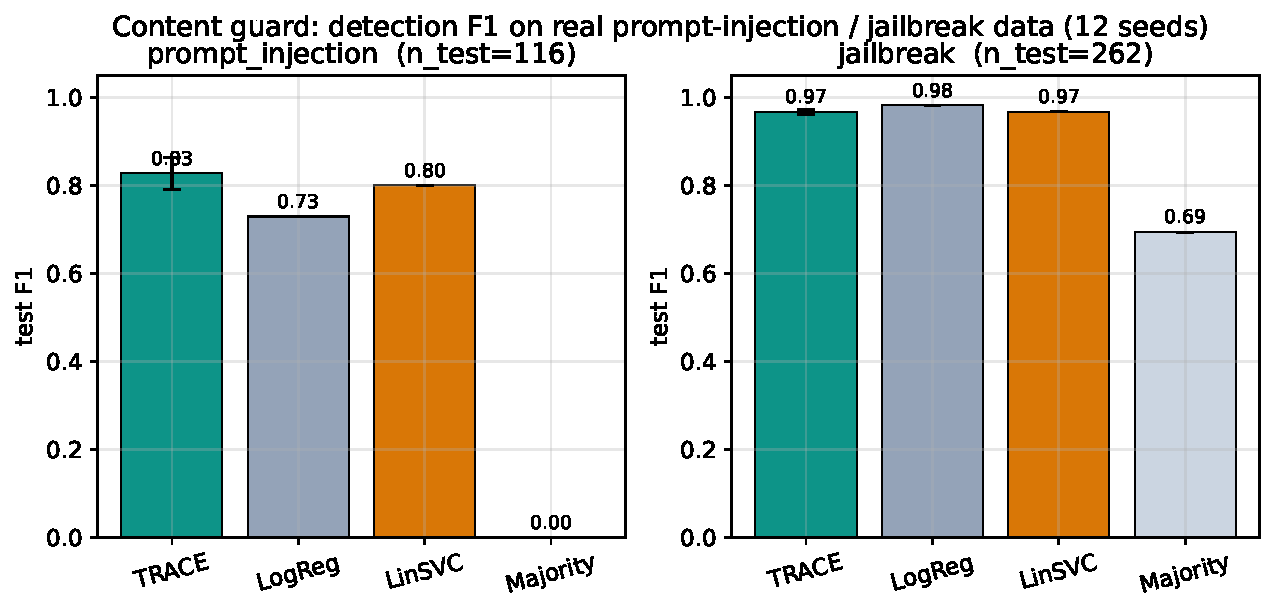
\includegraphics[width=0.95\linewidth]{figures/content_guard.pdf}
\caption{E1: detection F1 across models and datasets. TRACE significantly beats
the strongest CPU baseline on prompt-injection and is competitive on jailbreak,
at a fraction of the size and with human-readable clauses.}
\label{fig:content}
\end{figure}

\subsection{E2: Trajectory verification across four attack families}

I compare the \emph{per-call} (memoryless) paradigm, the regime every
per-request guardrail implements, against TRACE's online monitors on four
attack families grounded in the OWASP/Greshake taxonomy: slow-roll
\emph{exfiltration} (\textsc{BoundedCount}), out-of-role \emph{scope} violation
(\textsc{Always}), \emph{missing audit} of a sensitive read (\textsc{Response}),
and \emph{privilege} escalation (\textsc{Precedence}). The \texttt{scope} family
is deliberately single-step-visible. I report both attack success rate (ASR,
$=1-$detection) and false-positive rate (FPR) because together they expose a
\emph{fundamental bind} the memoryless paradigm cannot escape on temporal
properties (Table~\ref{tab:behavior}, Figure~\ref{fig:behavior}). On
\texttt{exfiltration} the per-call rule simply \emph{misses} the attack
(ASR $\btExfPcA$): every individual step is within role, so no stateless check
fires. On \texttt{missing\_audit} and \texttt{privilege} a stateless rule
\emph{can} flag the attack, but only by also flagging every benign session that
audits a step late or authorises before acting, driving FPR to $\btAudPcF$ and
$\btPriPcF$, i.e.\ useless in practice. Only on the single-step \texttt{scope}
family does the per-call rule work cleanly (ASR $\btScoPcA$, FPR $\btScoPcF$).
TRACE, carrying $O(1)$ bounded state, achieves ASR $0$ \emph{and} FPR
$\le \btAudTrF$ on \emph{all four} families: it matches the per-call paradigm
where memory is unnecessary and strictly dominates it (on either the ASR or the
FPR axis) everywhere memory is required.

\begin{table}[t]\centering\small
\caption{E2: attack success rate (ASR) and false-positive rate (FPR), both lower
is better, mean over 12 seeds. The memoryless per-call rule must trade one for
the other on the temporal families (\textbf{bold} = the failure: a missed attack
or a flag-everything FPR); TRACE keeps both near zero throughout.}
\label{tab:behavior}
\begin{tabular}{lcccccccc}
\toprule
& \multicolumn{2}{c}{exfiltration} & \multicolumn{2}{c}{missing\_audit}
& \multicolumn{2}{c}{privilege} & \multicolumn{2}{c}{scope} \\
\cmidrule(lr){2-3}\cmidrule(lr){4-5}\cmidrule(lr){6-7}\cmidrule(lr){8-9}
& ASR & FPR & ASR & FPR & ASR & FPR & ASR & FPR \\
\midrule
Per-call & $\mathbf{\btExfPcA}$ & \btExfPcF & \btAudPcA & $\mathbf{\btAudPcF}$
         & \btPriPcA & $\mathbf{\btPriPcF}$ & \btScoPcA & \btScoPcF \\
\textbf{TRACE} & \btExfTrA & \btExfTrF & \btAudTrA & \btAudTrF
         & \btPriTrA & \btPriTrF & \btScoTrA & \btScoTrF \\
\bottomrule
\end{tabular}
\end{table}

\begin{figure}[t]\centering
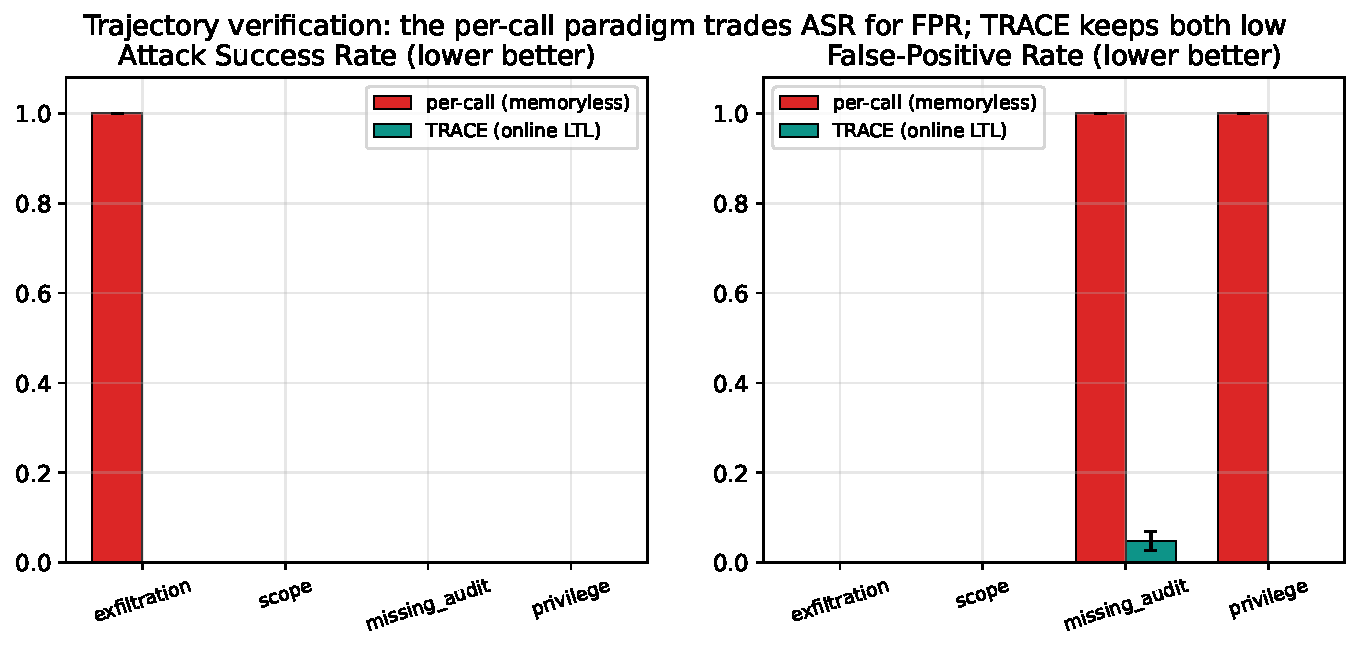
\includegraphics[width=0.92\linewidth]{figures/behavior_trajectory.pdf}
\caption{E2: ASR (left) and FPR (right) by attack family. The memoryless
paradigm either misses temporal attacks (exfiltration ASR) or flags every benign
session to catch them (missing\_audit, privilege FPR); TRACE's bounded-memory
monitors keep both low everywhere.}
\label{fig:behavior}
\end{figure}

\subsection{E3: Component ablation}

To show each channel earns its place, I build composite sessions whose threat
arrives on the content channel (a prompt injection drawn from the real test set),
the behaviour channel (a slow-roll exfiltration), both, or neither, and compare
content-only, behaviour-only, and combined TRACE. Averaged over the three attack
cells, content-only recall is $\ablContent$, behaviour-only is $\ablBehavior$,
and the combination is $\ablTrace$: each single channel is blind to the other's
attack, and only the combination covers both (Figure~\ref{fig:ablation}).

\begin{figure}[t]\centering
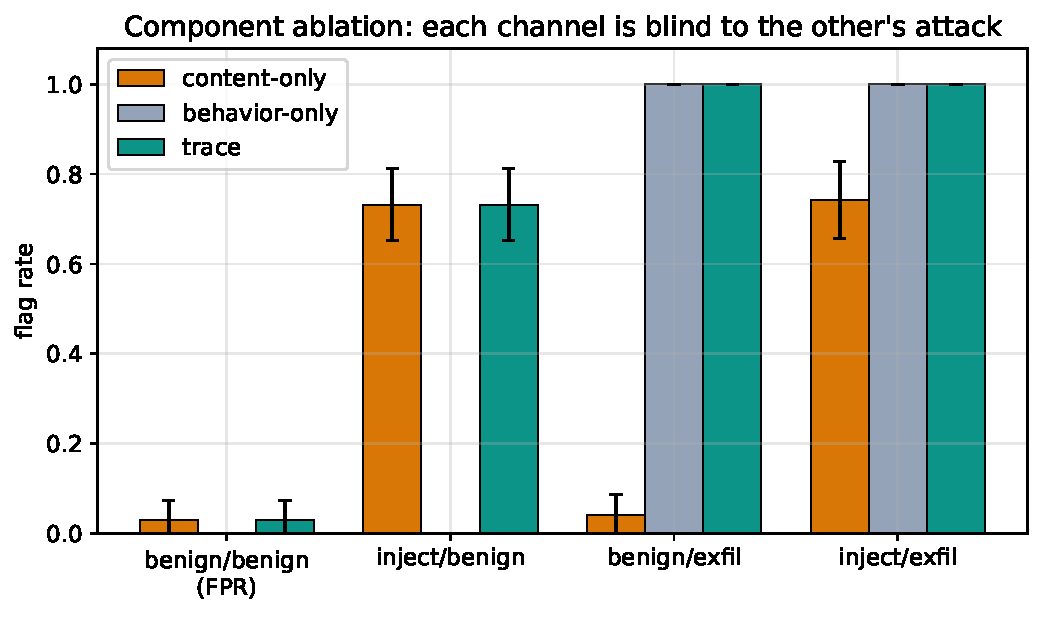
\includegraphics[width=0.85\linewidth]{figures/ablation.pdf}
\caption{E3: each channel detects only its own attack surface; TRACE's value is
the union.}
\label{fig:ablation}
\end{figure}

\subsection{E4: Tamper-evidence}

I seal mixed content/behaviour sessions and apply six tamper operations
(event flip, receipt-value flip, verdict edit, entry deletion, entry insertion,
reordering) plus a signature forgery without the key. Every class is detected at
rate $\tamperRate$ and localised: to the specific bad entry, or, when a tail
truncation leaves the forward chain intact, to the failing chain-head and
Merkle-root checks; untampered logs always verify; the forged signature (a valid
recomputed hash but no key) is caught by the per-entry HMAC check. Verification
costs $\verifyUs\,\mu$s for a typical session and scales
linearly in entries (Figure~\ref{fig:systems}, right). This is
Proposition~\ref{prop:tamper} in practice.

\subsection{E5: Systems characterisation}
\label{sec:systems}

Figure~\ref{fig:systems} reports the latency/accuracy/footprint trade-off. A
behaviour-guard step costs $\behLat\,\mu$s with $\behMem$\,bytes of monitor state;
the certificate ledger costs $\sim\ledgerBytes$ bytes per entry. Content-guard
latency grows linearly with the clause budget while F1 saturates, so a small
budget already buys most of the accuracy at sub-millisecond cost (median
$\latMed\,\mu$s, $99$th percentile $\latPNN\,\mu$s at the deployed $C{=}200$
budget). As an
\emph{order-of-magnitude} energy proxy (latency $\times$ an assumed $15$\,W CPU;
not a measurement, since I lack RAPL access) a content check draws on the order of a
millijoule; the measured endpoint of the TM hardware story is the
$8.6$\,nJ/frame ASIC of \citet{tunheim2025asic}, three orders of magnitude lower,
indicating substantial headroom for an edge deployment.

\begin{figure}[t]\centering
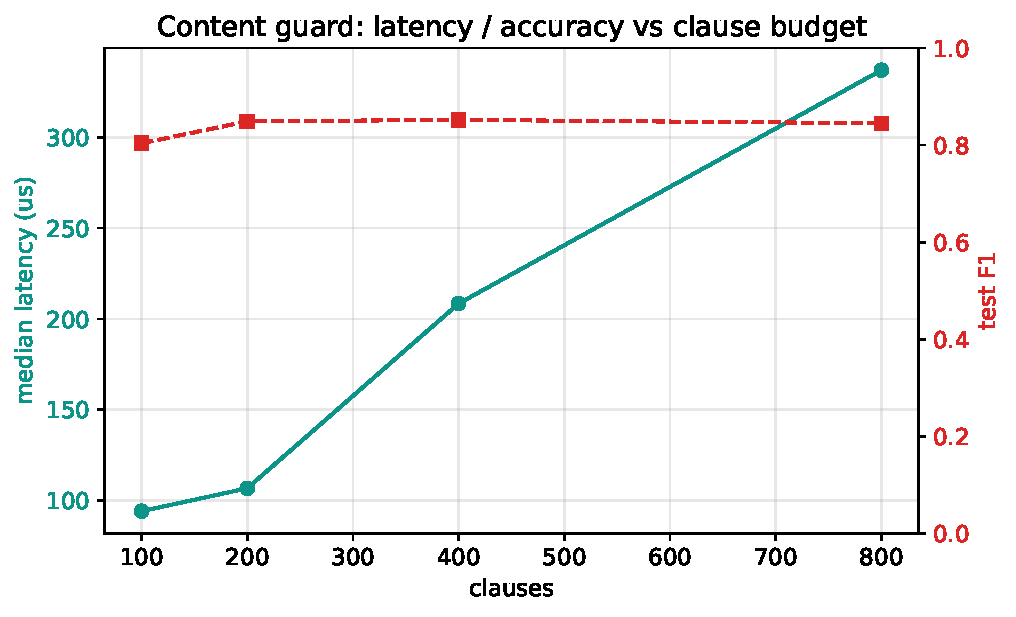
\includegraphics[width=0.49\linewidth]{figures/systems.pdf}\hfill
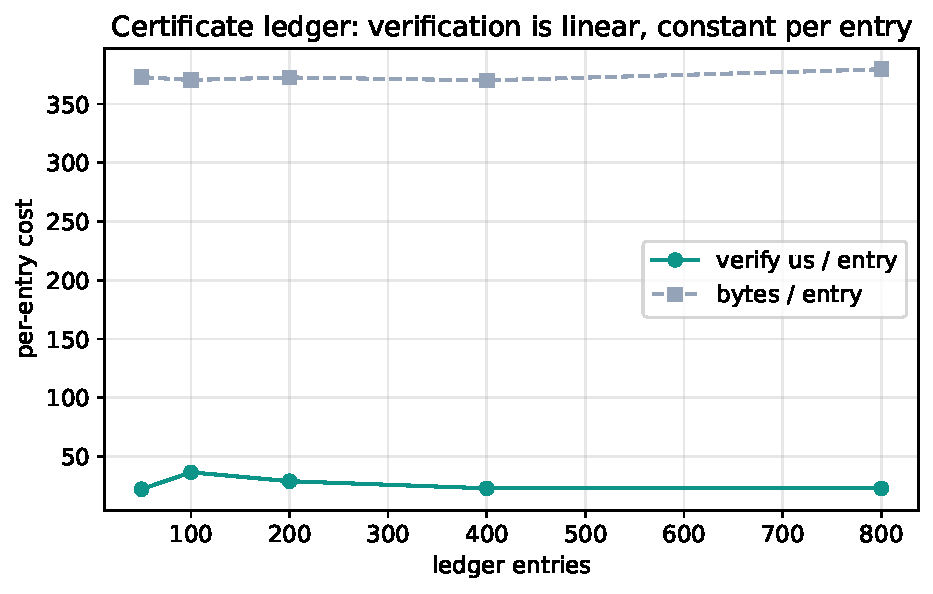
\includegraphics[width=0.49\linewidth]{figures/ledger_scaling.pdf}
\caption{E5: (left) content-guard latency and F1 vs clause budget; (right)
ledger verification is linear in entries at constant per-entry cost.}
\label{fig:systems}
\end{figure}

\subsection{E6: Robustness and honest failure modes}
\label{sec:robust}

Three probes, two of them deliberately adversarial to my own claims. First, an
\emph{adaptive} exfiltration attacker can only evade \textsc{BoundedCount}$(k{=}2)$
by staying at $\le 2$ exports: the monitor \emph{bounds the damage} rather than
being fooled (Figure~\ref{fig:adaptive}, left: detection is a clean step at the
budget). Second, surface \emph{obfuscation} of a fixed trigger lexicon
(character spacing, leetspeak, vowel repetition) barely moves recall
($\obfPlain$ plain $\to\obfSpace$ spaced): because the learned clauses key on a
broad token signal rather than a few keywords, this particular transform is
weak against TRACE, a mild robustness positive, though stronger semantic
paraphrase is untested and I make no claim there. Third, the real failure mode
is \emph{distribution shift}: a guard trained on one corpus and tested on the
other drops from $\transBin$ in-domain to $\transBcross$ cross-domain
($\transAin\!\to\!\transAcross$ in the reverse direction)
(Figure~\ref{fig:adaptive}, right), at or below chance, confirming the content
guard learns dataset-specific lexical cues and must be retrained per deployment.
Character-level literals and ensembling are the natural mitigations. I report
these rather than select against them.

\begin{figure}[t]\centering
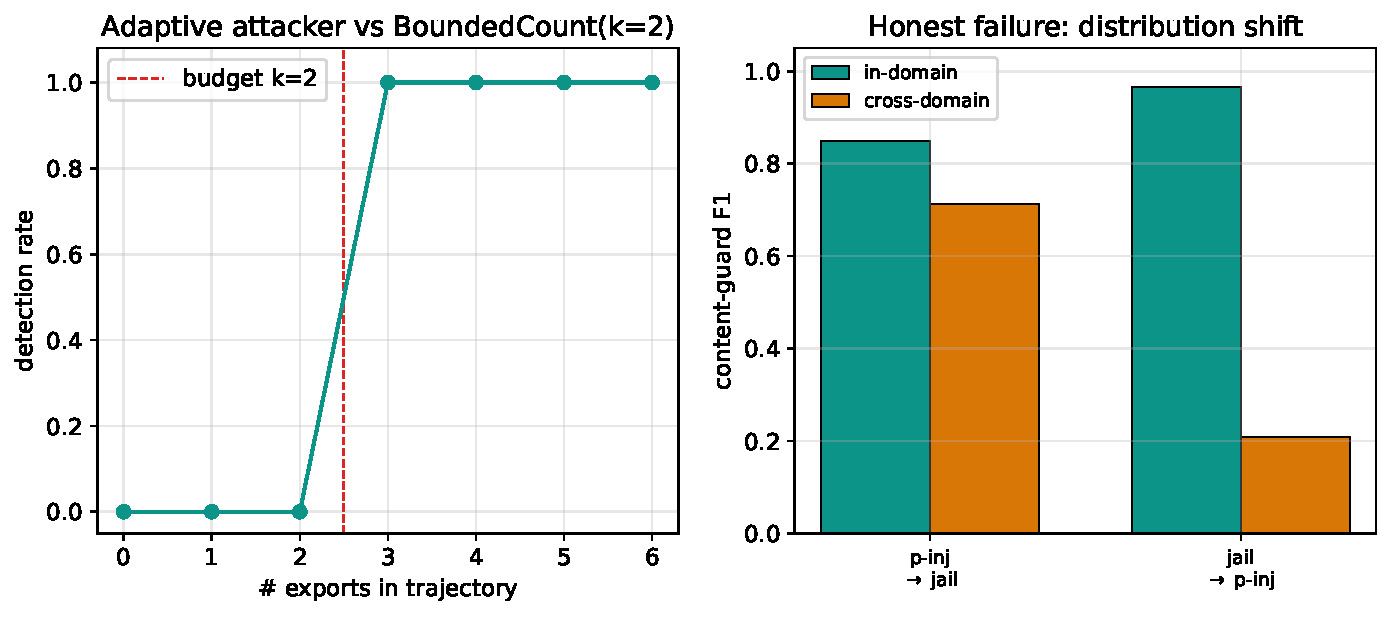
\includegraphics[width=0.95\linewidth]{figures/adaptive_robustness.pdf}
\caption{E6: (left) the temporal monitor forces an attacker under the rate budget,
bounding damage; (right) honest failure: the content guard's F1 collapses under
cross-dataset distribution shift.}
\label{fig:adaptive}
\end{figure}

\section{Discussion}

\paragraph{Positioning.} TRACE is, to my knowledge, the first guardrail to unify
five properties no incumbent offers more than two of: interpretability (readable
clauses vs an opaque forward pass), CPU-only sub-millisecond operation (vs
GPU-bound, latency-unspecified models), cryptographic auditability (vs no audit
trail anywhere in the survey), temporal-trajectory verification (vs per-call
classification), and cheap CPU retraining. Against the 2025 agent-enforcement
line~\citep{wang2025agentspec,wang2025proguard,kamath2025agentc} it is
distinguished by coupling enforcement with an interpretable learned detector and
a cryptographic session certificate, and by using deterministic constant-per-step
monitors. Relative to THGTM~\citep{debes2026thgtm}, which contributes the learned
detector substrate, TRACE is the end-to-end \emph{certifying runtime engine}: the
online monitor bank, the tamper-evident ledger, and the agentic framing are new.

\paragraph{When to use TRACE.} TRACE trades raw multilingual/multimodal detection
breadth for verifiable, auditable, edge-deployable assurance. It is the right
tool where a decision must be \emph{explained and certified}: regulated
deployments under the EU AI Act, on-device agents, or as a cheap, auditable first
stage in front of a heavier neural guardrail.

\section{Limitations and future work}
\label{sec:limits}
\begin{itemize}[leftmargin=1.4em]
\item \textbf{Learned-detector failure modes.} The content guard learns
dataset-specific lexical cues: cross-corpus F1 falls to near chance
(\S\ref{sec:robust}). Character-level literals, ensembling, and continual updates
are the natural fixes.
\item \textbf{Synthetic trajectory benchmark.} E2--E3 use synthetic trajectories
whose \emph{shapes} follow published taxonomies but are not drawn from a live
agent; validating on a multi-turn AgentDojo harness is future work.
\item \textbf{Declared-policy coverage.} The behaviour guard only catches
behaviours someone wrote a policy for; policy mining from logs is open.
\item \textbf{Symmetric authentication only.} The reference ledger is HMAC-based;
an Ed25519 signature over the Merkle root upgrades it to non-repudiation.
\item \textbf{Energy is a proxy.} I report a CPU energy proxy, not a measurement;
the ASIC endpoint is cited, not run.
\end{itemize}

\section{Ethics and broader impact}
This work is defensive. The trajectory benchmark is synthetic and contains no
personal data; the two text datasets are public and Apache-2.0. I disclose
TRACE's evasion modes (\S\ref{sec:robust}) precisely so deployers do not develop
a false sense of security: an auditable guardrail that is quietly bypassable is
worse than none if mistaken for complete. Positive impacts: a low-energy,
interpretable, certifiable guardrail lowers the cost of meeting emerging
auditability obligations and brings agent safety to CPU/edge settings. Negative
impacts: any guardrail can be over-trusted, and the interpretable clauses, while
auditable, also reveal the detector's logic to an adversary; I judge the
transparency benefit to outweigh this, consistent with open-source security
practice.

\section{Reproducibility}
The repository contains the library, 40 unit tests, the six experiments, the
figure script, the vendored datasets (pinned, Apache-2.0), and this paper's
source. \texttt{make test} runs the suite; \texttt{make reproduce} regenerates
every \texttt{results/*.json}; \texttt{make figures} rebuilds every figure;
\texttt{make paper} compiles this PDF. The host, seeds (12), all hyperparameters,
and the latency-measurement protocol are disclosed in \S\ref{sec:exp}.

\section{Conclusion}
TRACE shows that an agent guardrail need not be an opaque GPU model. Built on
propositional Tsetlin logic, it detects unsafe content with readable clauses,
verifies whole trajectories with online constant-memory temporal monitors, and
seals every session into a tamper-evident certificate an external auditor checks
without the model, at kilobytes and microseconds on a CPU. It is competitive
with, and on one real dataset significantly better than, strong CPU baselines for
detection, and it catches temporal attacks that the entire per-call guardrail
paradigm is structurally blind to. I am explicit about what it does not do.
What remains is validation on live agent harnesses, character-level robustness,
and an asymmetric-signature upgrade: each a concrete next step toward guardrails
that are not only effective but \emph{accountable}.

\paragraph{Reproducibility note.} Code, data, figures and this source live in the
TRACE repository; all experiments run with \texttt{make reproduce}.

\bibliography{references}
\end{document}
